\documentclass[runningheads]{llncs}
\usepackage{graphicx}
\usepackage{cite}
%\usepackage{hyperref}

\begin{document}

\title{Object-Oriented Internet\\ Cloud Interoperability}
\titlerunning{OOI - Cloud Interoperability}

\author{Mariusz Postół\inst{1}\orcidID{0000-0002-9669-0565}  \and Piotr Szymczak\inst{1}\orcidID{0000-0001-6790-3878} }
\authorrunning{M. Postół et al.}

\institute
{ Institute of Information Technology, Lodz University of Technology, Łódź, Poland \\
      \email{mailto:mariusz.postol@p.lodz.pl} %\\ \url{http://www.it.p.lodz.pl}
}

\maketitle

\begin{abstract}

      Optimization of the industrial processes requires further research on the integration of machine-centric systems with human-centric cloud-based services in the context of new emerging disciplines, namely Industry 4.0 and Industrial Internet of Things. This research aims at working out a new generic architecture and deployment scenario applicable to this integration. The reactive interoperability relationship of the interconnected nodes is proposed to deal with the network traffic propagation asymmetry or assets' mobility. Described solution based on the OPC Unified Architecture international standard relaxes issues related to the real-time multi-vendor environment. The discussion addressing the generic architecture concludes that the embedded gateway software part best suits all requirements. To promote separation of concerns and reusability, the proposed architecture of the embedded gateway has been implemented as a composable part of a selected OPC UA PubSub framework.

      The proposals are backed by proof of concept reference implementations confirming the possibility to integrate selected cloud services with the cyber-physical system interconnected as one whole atop of the OPC UA by applying the proposed architecture and deployment scenario. It is contrary to interconnecting cloud services with a selected OPC UA server limiting the PubSub role to data export only.

      \keywords{Industry 4.0 \and Internet of Things \and Object-Oriented Internet \and Cloud Computing \and Industrial communication \and Reactive Networking (RxNetworking)\and Machine to Machine Communication \and OPC Unified Architecture \and Azure}

\end{abstract}

\section{Introduction}\label{introduction}

All the time, the Information and Communication Technology is providing society with a vast variety of new distributed applications aimed at micro and macro optimization of the industrial processes. Obviously, the design foundation of this kind of application has to focus primarily on communication technologies. Based on the role humans take while using these applications they can be grouped as follows:

\begin{itemize}
      \item \textbf{human-centric} - information origin or ultimate information destination is an operator,
      \item \textbf{machine-centric} - information creation, consumption, networking, and processing are achieved entirely without human interaction.
\end{itemize}

A typical \textbf{human-centric} approach is a web-service supporting, for example, a web user interface (UI) to monitor conditions and manage millions of devices and their data in a typical cloud-based IoT approach. In this case, it is characteristic that any uncertainty and necessity to make a decision can be relaxed by human interaction. Coordination of robots behavior in a work-cell (automation islands) is a \textbf{machine-centric} example. In this case, any human interaction must be recognized as impractical or even impossible. This interconnection scenario requires the machine to machine communication (M2M) demanding multi-vendor devices integration.

From the M2M communication concept, a broader idea of a smart factory can be derived. In this M2M  deployment approach, the mentioned robots are only executive assets of an integrated supervisory control system responsible for macro optimization of an industrial process composed as one whole. Deployment of the smart factory concept requires a hybrid solution and interconnection of the mentioned above heterogeneous environments. This approach is called the fourth industrial revolution and was coined as Industry 4.0. It is worth stressing that machines - or more general assets - interconnection is not enough, and additionally, assets interoperability has to be expected for the deployment of this concept. In this case, multi-vendor integration makes communication standardization especially important, namely, it is required that the payload of the message is standardized to be factored on the data-gathering site and consumed on the ultimate destination site.

Highly-distributed solutions used to control real-time process aggregating islands of automation (e.g.~virtual power plants producing renewable energy) additionally must leverage public communication infrastructure, namely the Internet. Internet is a demanding environment for highly distributed process control applications designed atop the M2M communication paradigm because

\begin{itemize}
      \item it is a globally shareable and can be also used by malicious users
      \item it offers only non-deterministic communication making integration of islands of automation designed against the real-time requirements a difficult task
\end{itemize}

Today both obstacles can be overcome, and as examples, we have bank account remote control and voice over IP in daily use. The first application must be fine-tuned in the context of data security, and the second is very sensitive in regard to time constraints. Similar approaches could be applied to adopt the well known in process control industry concepts:

\begin{itemize}
      \item  Human Machine Interface (HMI)
      \item Supervisory Control and Data Acquisition (SCADA)
      \item Distributed Control Systems (DCS)
\end{itemize}

A detailed examination of these solutions is far beyond the scope of this article. It is only worth stressing that, by design, all of them are designed on the foundation of interactive communication. Interactive communication is based on a data polling foundation. In this case, the application must follow the interactive behavioral model, because it actively polls the data source for more information by pulling data from a sequence that represents the process state in time. The application is active in the data retrieval process - it controls the pace of the retrieval by sending the requests at its convenience. Such a polling pattern is similar to visiting the books shop and checking out a book. After you are done with the book, you pay another visit to check out another one. If the book is not available you must wait, but you may read what you selected. The client/server archetype is well suited for the mentioned above applications.

After dynamically attaching a new island of automation the control application (responsible for the data pulling) must be reconfigured for this interoperability scenario. In other words, in this case, the interactive communication relationship cannot be directly applied because the control application must be informed on how to pull data from a new source. As a result, a plug and produce scenario \cite{PlugProduceByModellingSkills} cannot be seamlessly applied. A similar drawback must be overcome if for security reasons suitable protection methods have been applied to make network traffic propagation asymmetric. It is accomplished using intermediary devices, for example, firewalls, to enforce traffic selective availability based on predetermined security rules against unauthorized access.

Going further, we shall assume that islands of automation are mobile, e.g.~autonomous cars passing a supervisory controlled service area. In this case, the behavior of the interconnected assets is particularly important concerning the environment in which they must interact. This way we have entered the Internet of Things domain of Internet-based applications.

If we must bother with the network traffic propagation asymmetry or mobility of the asset network attachment-points the reactive relationship could relax the problems encountered while the interactive approach is applied. In this case, the sessionless publisher-subscriber communication relationship is a typical pattern to implement the abstract reactive interoperability paradigm. The sessionless relationship is a message distribution scenario where senders of messages, called publishers, do not send them directly to specific receivers, called subscribers, but instead, categorize the published messages into topics without knowledge about which subscribers if any, there may be. Similarly, subscribers express interest in one or more topics and only receive messages that are of interest, without knowledge about which publishers, if any, there are. In this scenario, the publishers and subscribers are loosely coupled i.e they are decoupled in time, space and synchronization \cite{RefWorks:doc:5c44e246e4b0591b15ea9e59}.

If the \textbf{machine-centric} interoperability - making up islands of automation - must be monitored and/or controlled by a supervisory system cloud computing concept may be recognized as a beneficial solution to replace or expand the mentioned above applications, i.e.~HMI, SCADA, DCS, etc. Cloud computing is a method to provide a requested functionality as a set of services. There are many examples that cloud computing is useful to reduce costs and increase robustness. It is also valuable in case the process data must be exposed to many stakeholders. Following this idea and offering control systems as a service, there is required a mechanism created on the service concept and supporting abstraction and virtualization - two main pillars of the cloud computing paradigm. In the cloud computing concept, virtualization is recognized as the possibility to share the services by many users, and abstraction hides implementation details.

Deployment of the hybrid solution providing interoperability of the \textbf{machine-centric} Cyber-Physical System (CPS) and \textbf{human-centric} cloud-based front-end can be implemented applying the following scenarios: \textbf{direct} or \textbf{gateway} based interconnection (Sect. \ref{subs.architecture}).

By design, the \textbf{direct} approach requires that the cloud has to be compliant with the interoperability standard the CPS is built upon - it becomes a consistent part of the CPS. Data models, roles, and responsibility differences of both solutions make this approach impractical or even imposable to be applied in typical cases. A more detailed description is covered by the Sect.~\ref{cloud-to-sensors-field-level-connectivity}.

This article addresses further research on the integration of the multi-vendor \textbf{machine-centric} CPS designed atop of M2M communication and emerging cloud computing as a \textbf{human-centric} front-end in the context of the Industry 4.0 (I4.0) and Industrial Internet of Things (IIoT) disciplines. For this integration, a new architecture is proposed to support the reactive relationship of communicating parties. To support the multi-vendor environment OPC Unified Architecture \cite{LiteratureSurveyOnOpenPlatformCommunications} interoperability standard has been selected. Prototyping addresses Microsoft Azure Cloud as an example. The proposals are backed by proof of concept reference implementations - the outcome has been just published on GitHub as the open-source (MIT licensed) \cite{mariusz_postol_2020_4361640}. The proposed solutions have been harmonized with the more general concept called the Object-Oriented Internet \cite{mariusz_postol_2020_4361640}.

The main goal of this article is to provide proof that:

\begin{enumerate}
      \item  reactive interoperability M2M communication based on the OPC UA standard can be implemented as a powerful standalone library without dependency on the Client/Server session-oriented archetype
      \item Azure interoperability can be implemented as an external part employing out-of-band communication without dependency on the OPC UA implementation
      \item the proposed generic architecture allows that the gateway functionality is implemented as composable part at run-time part - no programming required
\end{enumerate}

The remainder of this paper is structured as follows. Sect.~\ref{cloud-to-sensors-field-level-connectivity} presents the proposed open and reusable software model. It promotes a reactive interoperability pattern and a generic approach to establishing interoperability-context. A reference implementation of this archetype is described in Sect.~\ref{sect.gateway-implementation}. The most important findings and future work are summarized in Sect.~\ref{section.conclusion}.

\section{Sensors to Cloud Field Level Connectivity}\label{cloud-to-sensors-field-level-connectivity}

\subsection{Architecture}\label{subs.architecture}

As it was explained in Sect.~\ref{introduction}, to follow the Industry 4.0 concept a hybrid environment integrating reactive Machine to Machine interconnection and the interactive web-based user interface is required (Sect. \ref{introduction}). The main challenge of the solution in concern is to design a generic but reusable architecture that addresses interoperability of these diverse interconnection scenarios ruled by different requirements, namely:

\begin{enumerate}
      \item \textbf{machine-centric} machine to machine real-time mobile interoperability
      \item \textbf{human-centric} cloud-based front-end
\end{enumerate}

Interconnection of the reactive \textbf{machine-centric} and interactive \textbf{human-centric} environments can be implemented by applying one of the following scenarios:

\begin{itemize}
      \item \textbf{direct interconnection} (tightly coupled scenario) - cloud-based dedicated communication services are engaged to attach it to the CPS making up a consistent M2M communication network using a common protocol stack
      \item \textbf{gateway based interconnection} (loosely coupled scenario) - native build-in communication services allows attaching the cloud to the CPS using an out-of-bound protocol stack
\end{itemize}

In the solution in concern, the interconnection of assets is not enough  hence their interoperability is expected. In this case, using the same communication stack must be recognized as only a necessary condition. To support interoperability common data understanding is required. By design, the direct approach requires that the cloud has to be compliant with the interoperability standard the CPS uses. As a result, it becomes a consistent communication node of the CPS. Additionally, to meet this requirement the cloud and CPS have to establish directly the same:

\begin{itemize}
      \item semantic-context
      \item security-context
\end{itemize}

The possibility to establish a common semantic-context in the multi-vendor environment makes communication standardization especially important. In this case, it is required that the encoding of the payload exchanged over the network (Data Transfer Object - DTO) is standardized so that the appropriate messages can be factored on the data-gathering site and consumed on the ultimate destination data processing sites. Security between the data origin and ultimate data destination refers to the protection of messages (security-context) against malicious users. It is required that communicating parties are using the same cyber-security measures.

The decision to follow the \textbf{direct interconnection} scenario must be derived from an analysis of the capabilities of available services in concern. However, for the development strategy of this type of solutions this analysis can be done partially taking into account two features that can be considered invariable:

\begin{itemize}
      \item by design the cloud-based services must be virtual - they are used to handle many solutions at the same time
      \item by design the M2M communication is usually constrained by the real-time requirements
\end{itemize}

The virtualization of cloud services means that they must be very flexible to handle the attachment of new assets proactively (acting in advance) at run time. As a result, by design, the cloud services must be responsible to register and authenticate devices by exposing endpoints in the public network to allow the device to access a provisioning cloud service. It requires that a session over the Internet has to be established by the data holding asset at a preparation step.

To meet the requirements of real-time distributed control the CPS may use protocols applicable only to local computer networks (e.g.~multicast IP, Ethernet, TSN \footnote{Time-Sensitive Networking (TSN) Task Group \url{https://1.ieee802.org/tsn/}}, etc.). Because the cloud services support only protocols handling interconnection over the Internet the interaction with the cloud requires remote agents, i.e.~agents attached locally to the M2M network and implemented by applying one of the following archetypes:

\begin{itemize}
      \item \textbf{edge device} - remote cloud agent acting as an intermediary for nodes of the CPS
      \item \textbf{field level gateway} - a dedicated custom agent acting as an intermediary for nodes of the CPS
      \item \emph{Embedded Gateway} - a software part composed into a selected node of the \emph{Cyber-physical network} (\ref{figure1.StrategyDomainModel})
\end{itemize}

\begin{figure}
      \centering
      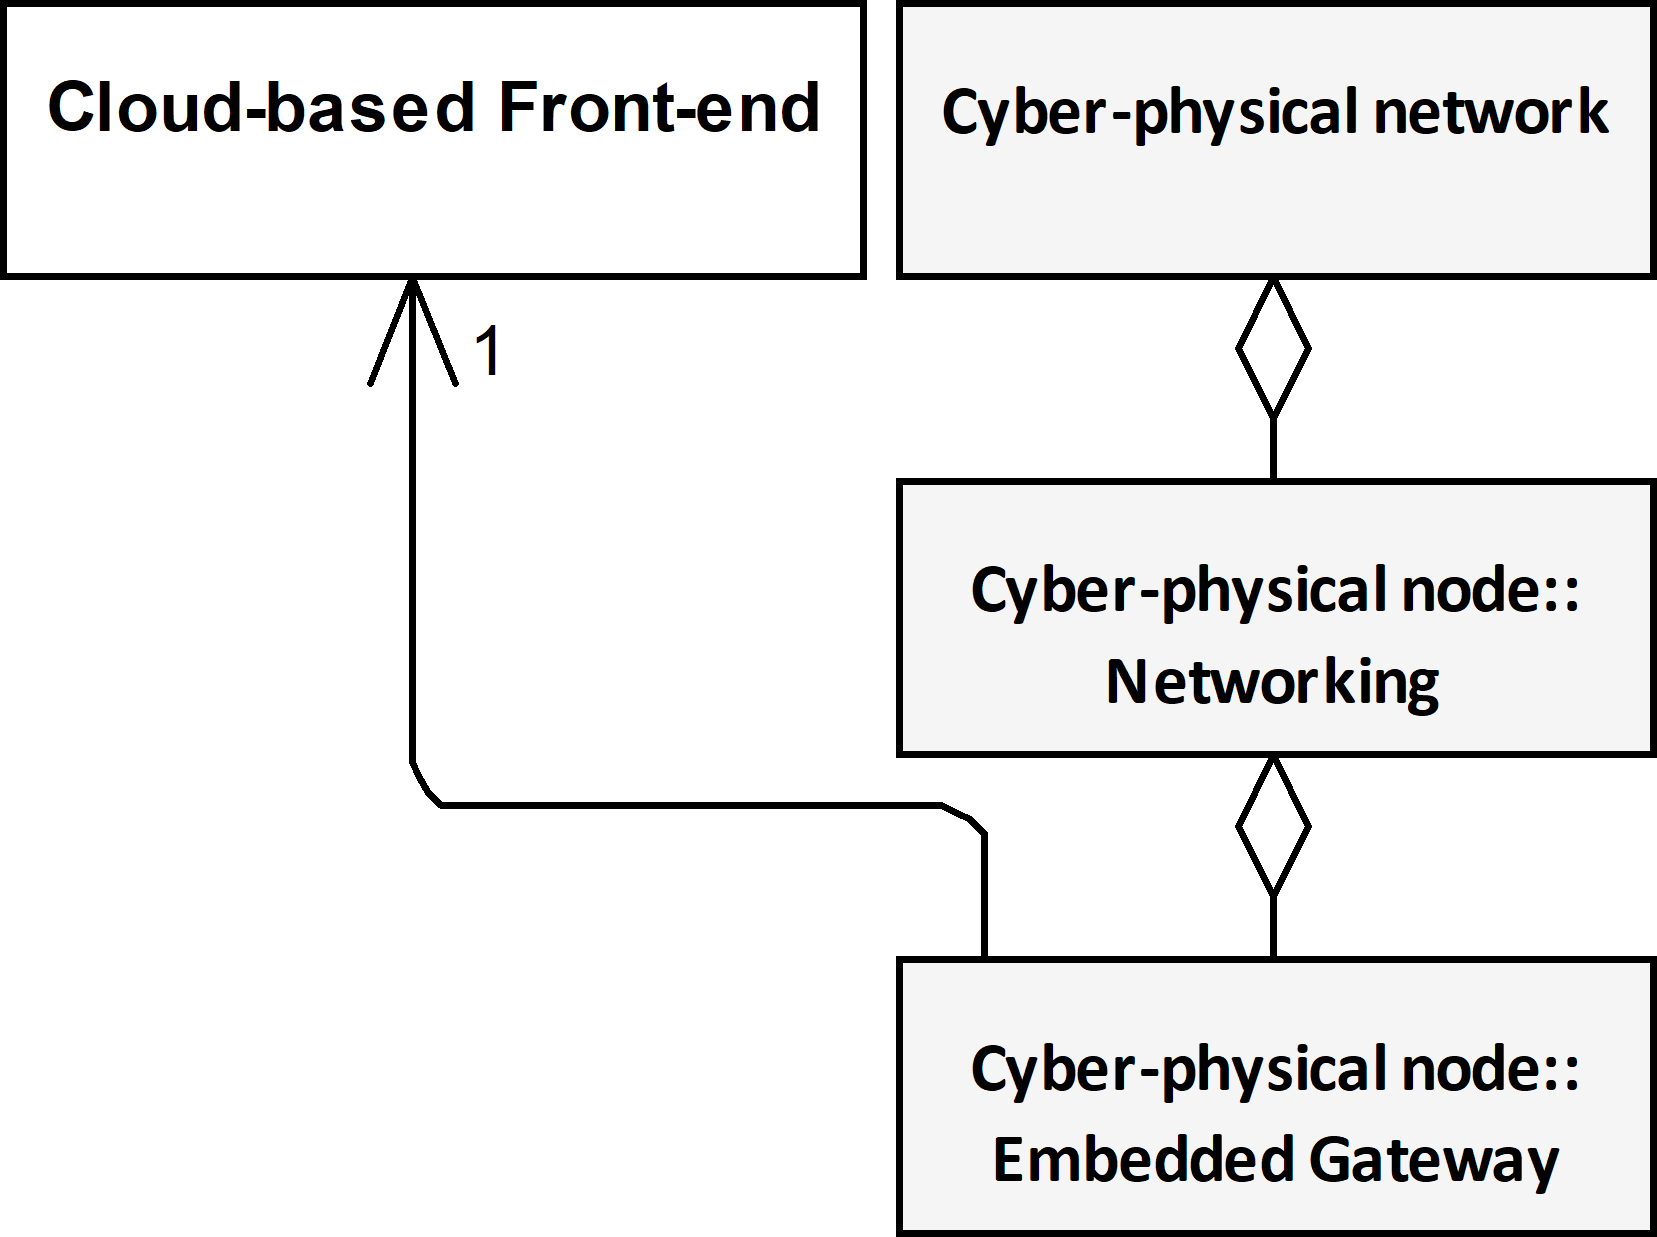
\includegraphics[width=8cm]{../../.Media/StrategyDomainModel.png}
      \caption{Domain model of a generic interconnection concept}\label{figure1.StrategyDomainModel}
\end{figure}

\textbf{Edge device} connects directly to the cloud services but acts as an intermediary for other devices called leaf devices. Additionally, it allows the selection of initial data processing and execution of them using local resources. The \textbf{edge device} may be located close to the leaf devices and attached to the \emph{Cyber-physical network} using protocols applicable only to local computer networks. In this scenario, it is possible to use a custom protocol stack to get connected to the \textbf{edge device} with the cloud and helps to save the bandwidth thanks to sending only the results of local processing. In this approach, the \textbf{edge device} is part of cloud vendor products and cannot be recognized as a generic solution that can be used to connect to other clouds at the same time.

The \textbf{field level gateway} is also build atop of the middleware concept \cite{Sunyaev2020}. The only difference compared with the \textbf{edge device} is a necessity to use officially supported by the cloud vendor services to get connected. In this scenario, the process data simultaneously may be transferred to many clouds provided that the gateway offers this functionality.

Unlike the above-described solutions, the \emph{Embedded Gateway} is not derived from the middleware concept. A generic domain model for this interconnection is presented in the Fig.~\ref{figure1.StrategyDomainModel}. Promoting separation of concern design principle, the gateway functionality should be implemented as a self-contained software part embedded in the \emph{Networking} service of the \emph{Cyber-physical\ node}. The main functionality of this component is to transfer selected data between \emph{Cyber-physical\ network} using \emph{Networking} services of an existing \emph{Cyber-physical\ node} and \emph{Cloud-based\ front-end} using officially supported by the cloud vendor interconnection services.

The \emph{Embedded Gateway} archetype relaxes most of the issues described above: \emph{Cyber-physical\ network} real-time behavior, data encoding incompatibility, security - context differences to name only a few. The main goal of this article is to provide proof that the \emph{Embedded Gateway} archetype implementation is possible based on a generic architecture that can be used as a foundation for the integration of the heterogeneous environments in concern. The proposed implementation is designed for a selected interoperability standard and cloud product.

To comply with the Industry 4.0 communication criterion it is required that any product must be addressable over the network via TCP/UDP or IP and has to support the OPC UA Information Model. As a result, any product being advertised as Industry 4.0 enabled must be OPC UA-capable somehow. To support the multi-vendor environment OPC Unified Architecture interoperability standard has been selected. OPC UA supports the following two patterns to be used to transfer data between communicating parties:

\begin{itemize}
      \item \textbf{session-oriented}: requires a session that has to be established before any data can be sent between sender and receiver
      \item \textbf{sessionless-oriented}: the sender may start sending messages (called packets or datagrams) to the destination without any preceding handshake procedure
\end{itemize}

Using the session-oriented communication pattern it is difficult or even impossible to gather and process mobile data (Sec.~\ref{introduction} ), which is one of the Internet of Things paradigms. OPC UA Part 14 PubSub \cite{RefWorks:doc:5d98837de4b055984c0eecf0, UAPart14PubSubMainTechnologyFeatures} offers the sessionless approach as an additional option to session-based client-server interoperability relationship and is a consistent part of the OPC UA specifications suit. As the result, it can be recognized as the IoT ready technology.


The presented proposals in the article are backed by proof of concept reference implementations\cite{mariusz_postol_2020_4361640}. For this study, prototyping addresses Microsoft Azure cloud products. There are many reasons for selecting Azure to accomplish the cloud-based front-end of Cyber-Physical System (CPS). Azure offers Infrastructure as a Service (IaaS) and Platform as a Service (PaaS) capabilities. As a result, the platform can be used not only as a cloud-based front-end for CPS. By design, the Azure services are compliant with Security Development Lifecycle (SDL) an industry-leading security process. It is also compliant with the new international standard for cloud privacy, namely ISO 27018. Solutions hosted on Azure are scaled up to millions of users without any additional coding. For the development of the CPS front-end, it is essential that Azure provides very efficient storage services usefully for the purpose of real-time process data archival. Azure provides a vast variety of hybrid connections including but not limited to virtual private networks (VPNs), caches, content delivery networks (CDNs), ExpressRoute, and IoT dedicated services that can be directly used to implement cloud-based front-end for CPS. Because it is also integrated with other Microsoft tools like Office 365, Outlook, and SharePoint using Azure allows preserving investment and exporting process data to the mentioned tools. Azure also offers services supporting analytics and intelligence capabilities for further improving business processes and decision making. It is the only cloud platform that offers Blockchain as a Service (BaaS), Machine Learning, Bots, and Cognitive APIs capabilities.

Azure aids Internet protocols and open standards such as JSON, XML, SOAP, REST, MQTT, AMQP, and HTTP. A software development kits for C\#, Java, PHP, and Ruby are available for custom applications. Azure provides services supporting data exchange over the OPC UA, but they don't support PubSub compliant with the OPC UA Part-14. Connectivity services on the network use JSON-based Data Transfer Object encoded based on schema derived from the solution metadata.

A more detailed description of the selected Azure features in the context of the application in concern is covered by the Sec.~\ref{azure-main-technology-features}.

Based on the sessionless and session-oriented communication patterns examination against the IoT requirements \cite{mpostol2020} it could be concluded that the connectionless pattern better suites issues related to the assets mobility and traffic asymmetry that is characteristic for the application domains in concern. Additionally, to promote interoperability and address the demands of the M2M communication in the context of a multi-vendor environment the prototyping should use a framework that must be compliant with the OPC UA Part 14 PubSub  specification. According to proposed generic architecture (Fig.~\ref{figure1.StrategyDomainModel}) to implement the \emph{Embedded\ Gateway} as a composable part of the \emph{Cyber-physical\ node} a library implementing \emph{Networking} functionality in compliance with mentioned above specification is a starting point for further development. Additionally, it must be assumed that the library used to deploy \emph{Embedded\ Gateway} support dependency injection and be capable to compose an external part supporting Azure/PubSub gateway functionality. The composition process must be available without modification of the core code of an existing library. As a result, the prototyping is to be limited to implementation of the \emph{Embedded\ Gateway} software part only.

A library that meets all these requirements has been implemented consistently with the Object-Oriented Internet paradigm \cite{mariusz_postol_2020_4361640} worked out in an open-source project \footnote{ \url{https://github.com/mpostol/OPC-UA-OOI} }. The paper \cite{mpostol2020} covers the description of a reference application program implementation proving that it is possible to design universal architecture targeting reactive interoperability as a consistent part of the Object-Oriented Internet concept compliant with the OPC UA PubSub international standard. According to the presented implementation and evaluation, using the dependency injection and late binding, the application program can be seamlessly adapted to the production environment and scales well. This approach also improves flexibility and adaptability of the existing solutions against any modification of the production environment, including but not limited to the selected interoperability standard change.

Sect.~\ref{ooi-main-technology-features} provides a more detailed description of this library and an external part deployment process that is to be used to implement new functionality supporting \emph{Embedded\ Gateway}.

The following subsections cover the description of the current state of technologies concerning Azure cloud-based IoT enabler and OPC UA PubSub. Sect. \ref{azure-main-technology-features} analyzes data presentation user interface, available native communication services, and data/metadata model offered by Microsoft Azure. The discussion covered by this section is the foundation for selecting services utilized to expose process data and suitable protocol stack to support interconnection. In Sect. \ref{ooi-main-technology-features} the discussion focuses on the generic architecture that is to be used as a foundation for further decisions addressing the systematic design of the interoperability of the CPS and cloud-based front-end.



\subsection{Azure Main Technology Features}\label{azure-main-technology-features}

Deployment of the hybrid solution providing interoperability of the \textbf{machine-centric} Cyber-Physical Systems (CPS) designed atop of M2M reactive communication and emerging cloud computing as a \textbf{human-centric} front-end requires decisions addressing the selection of the services supporting web user interface capable to expose process data. In this context, the service is any autonomous (with its own identity) software component or module that is interfacing with selected CPS for data collection, analysis, and also remote control. Microsoft Azure is a cloud-based product. It offers a vast variety of services. This virtual environment handles an unlimited number of users and devices organized using a solution container concept. The solution aggregates users, devices, services, and required additional resources scoping on a selected scenario. It also serves as a context that provides a scope to the identifiers (the names of devices, users, process data entities, etc) inside it. Solutions are used to organize deployment entities into logical groups and prevent identity collisions.

The \textbf{IoT\ Central} service provides a user interface of process data visualization. To make this interface meaningful, metadata called device template is used to describe devices.

Following the assumption that interconnection between the CPS and cloud services is designed based on the gateway concept, a middleware must be considered as a coupler. It must be interconnected with the CPS using an in-band protocol adhering to communications requirements (i.e. protocol profile, data encoding, time relationships, etc.) governing communication of the parts making it up. At the same time, it must support back-and-forth data transfer to the cloud using out-of-band native for the cloud services. The transfer process requires data conversion from source to destination encoding. The \textbf{IoT\ Hub} is a service hosted in the cloud that supports \textbf{IoT\ Central} services providing a robust messaging solution - it acts as a central message hub for bi-directional communication \cite{MicrosoftAzureIoTPlatform}. This communication is transparent, i.e.~it is not data types aware allowing any devices to exchange any kind of data. This service is responsible to manage the devices' identity and it offers the following protocol stacks: AMQP, MQTT, and HTTPS.


Before process data can be exposed using a web user interface the data source must be associated with an appropriate solution and validated to make sure that the security rules are not violated. It is hard to assume that the security rules governing the CPS may also apply to the cloud-based services. In the gateway scenario, they can be mapped on each other or be entirely independent. The \emph{IoT\ Hub\ Device\ Provisioning\ Service} (DPS) is a helper service for \emph{IoT\ Hub} that enables devices' connection process management, upon device providing valid identity attestation it assigns the device to an appropriate \emph{IoT\ Hub} instance and returns to the device connection parameters, which allow direct connection with given \emph{IoT\ Hub} service. The device proceeds to use the same attestation in \emph{IoT\ Hub} connection and based on it, is granted authorization to selected operations including but not limited to data transfer and updating the user interface.

It is worth stressing that interaction of the offered by the Azure services can be configured flexibly, and as a result, the presented above selection of services must be recognized as an example only. The \textbf{IoT\ Central} can be also seamlessly integrated with other services as needed. The following services could also be considered to build a cloud-based automation solution:

\begin{itemize}
      \item \emph{Industrial\ IoT} - discovering OPC UA enabled servers in a factory network and register them in Azure \emph{IoT\ Hub} implemented using \emph{IoT\ Edge}
      \item \emph{Digital\ Twins} - managing the graph of digital twins, which are to represent some real-world process or entity
\end{itemize}


\emph{Industrial\ IoT} promotes OPC UA client/server archetype used to achieve direct and interactive interoperability implemented using \emph{IoT\ Edge} services that allow extracting initial data processing to local premises based on the edge concept. \emph{Digital\ Twins} is an emerging concept to use an observer to replicate selected process state and behavior. The possibility to add value as a result of using these services must be subject to further research.

\subsection{OOI Main Technology Features}\label{ooi-main-technology-features}

subsection

\section{Azure - Object-Oriented Internet Interoperability Implementation}\label{sect.gateway-implementation}

section

\section{Conclusion}\label{section.conclusion}

section

\bibliography{ICCS21MPostoOOIGateway2Azure}
\bibliographystyle{splncs04}

\end{document}
